% Copyright 2021 Joel Feldman, Andrew Rechnitzer and Elyse Yeager, except where noted.
% This work is licensed under a Creative Commons Attribution-NonCommercial-ShareAlike 4.0 International License.
% https://creativecommons.org/licenses/by-nc-sa/4.0/

\section*{3.2: Related Rates}

\begin{frame}{Table of Contents}

\mapofcontentsC{\cb}
\end{frame}

%----------------------------------------------------------------------------------------
%----------------------------------------------------------------------------------------
%----------------------------------------------------------------------------------------
%----------------------------------------------------------------------------------------


\begin{frame}{Related Rates - Introduction}
``Related rates" problems involve finding the rate of change of one quantity, based on the rate of change of a related quantity.


\includegraphics[height=2cm]{Clipart/gears}
\index{
\includegraphics[height=5mm]{Clipart/gears}
\href{https://thenounproject.com/term/gears/73806/}{`Gears'} by 
\href{https://thenounproject.com/DHETTEIX/}{Dan Hetteix} is licensed under
 \CCBYthree~ (accessed 7 July 2021)}

\note{As usual, there are more examples here than you'll probably get to in class.}
\end{frame}
%----------------------------------------------------------------------------------------
\begin{frame}[t]
\unote{Example~\eref{text}{eg:percentGrowth}}
\only<1>{\QuestionBar{1}{9}\AnswerYes}
\only<2>{\AnswerBar{1}{9}}
Suppose $P$ and $Q$ are quantities that are changing over time, $t$. Suppose they are related by the equation \[3P^2=2Q^2+Q+3.\] If $\dfrac{dP}{dt}(t)=5$ 
when $P(t)=1$ and $Q(t)=0$, then what is $\dfrac{dQ}{dt}$ at that time?\pause\color{answercolor}

\vfill
\answer{
Apply $\diff{}{t}$ to both sides of $3P(t)^2=2Q(t)^2+Q(t)+3$.
\begin{align*}
6P(t)\frac{dP}{dt}(t)&=4Q(t)\frac{dQ}{dt}(t)+\frac{dQ}{dt}(t)
\end{align*}
Then when $\dfrac{dP}{dt}(t)=5$,  $P(t)=1$ and $Q(t)=0$,
\begin{align*}
6(1)(5)&=4(0)\frac{dQ}{dt}+\frac{dQ}{dt}\\
30&=\frac{dQ}{dt}
\end{align*}}
\end{frame}
%----------------------------------------------------------------------------------------

\begin{frame}[t]
\begin{center}\color{C3}
Related rates problems often involve some kind of geometric or trigonometric modeling
\end{center}
\QuestionBar{2}{9}\AnswerYes



A garden hose can pump out a cubic meter of water in about 20 minutes. Suppose you're filling up a rectangular backyard pool, 3 meters wide and 6 meters long, with a garden hose. How fast is the water rising?
\end{frame}
%----------------------------------------------------------------------------------------
\begin{frame}<handout:0>[t]
\AnswerBar{2}{9}
\color{answercolor}
We know the rate of change over time of the volume of water, and we want to know the rate of change over time of the height of the water.

\bigskip
 Let $V$ be the volume of water in the cell, and let $h$ be the height of water. Then we relate $V$ and $h$:
\[V = 3 \cdot 6 \cdot h = 18h\]
where $V$ is measured in cubic meters, and $h$ is measured in meters. Then we differentiate both sides with respect to $t$:
\[\frac{dV}{dt} = 18\frac{dh}{dt}\]
Now, $\frac{1}{20} = 18\frac{dh}{dt}$, so the water level is rising at about $\frac{1}{20\cdot 18} = \frac{1}{360}$ meters per minute, or something less than a third of a centimeter per minute. It's going to take a long time to fill up the pool.
\end{frame}
%----------------------------------------------------------------------------------------
\begin{frame}{Solving Related Rates}
1. Draw a Picture
\vfill

2. Write what you know, and what you want to know. Note units.\vfill

\color{M4}3. Relate all your relevant variables in one equation.\vfill\color{black}

4. Differentiate both sides (with respect to the appropriate variable!)\vfill

5. Solve for what you want.

\note{Repeat in class: ``If we know how to things are related, we can differentiate to find how their derivatives are related."

For the first few examples, the answers are given with this structure. After that, it's more condensed. Students will likely appreciate if you (at least verbally) continue mentioning these steps, but at some point it's good to leave them and let students develop a little more flexibility and confidence.}
\end{frame}

%----------------------------------------------------------------------------------------
%----------------------------------------------------------------------------------------
\begin{frame}[t]
\QuestionBar{3}{9}\AnswerYes\MoreSpace
A weight is attached to a rope, which is attached to a pulley on a boat, at water level. The weight is taken \textcolor{C3}{8 (horizontal) metres} from its attachment point on the boat, then dropped in the water. 

The weight sinks straight down. The rope stays taught as it is let out at a constant rate of \textcolor{C3}{one metre per second}, and \textcolor{C3}{two seconds} have passed. How fast is the weight descending?

\begin{center}
\begin{tikzpicture}[yscale=0.5]

\begin{scope}
\clip (-1,0.5) rectangle (5,-4.5);
\shadedraw[C4, shading=axis, top color=C4!70, bottom color=C1!70,ultra thick, decorate, decoration=snake ](-1.5,0) rectangle (5.5,-5);
\end{scope}

\draw (1,.1) node(a)[rotate=45]{
\includegraphics[width=4mm]{Clipart/switch}};
\draw (4,-3) node[vertex](c){};
\draw (a)--(4,-3);
\draw[decorate,decoration={brace, amplitude=10pt}](1,.75)--(4.2,.75) node[midway, above, yshift=10pt]{8};
\draw[densely dashed, thick, ->] (4,-3.5)--(4,-4.4);
\end{tikzpicture}
\end{center}
\index{
\includegraphics[height=5mm]{Clipart/switch} 
\href{https://thenounproject.com/term/switch/40327/}{`Switch'} by 
\href{https://thenounproject.com/kstaelin/}{K Staelin} is in the
public domain (accessed 7 July 2021)}

\end{frame}
%----------------------------------------------------------------------------------------%----------------------------------------------------------------------------------------
\begin{frame}<handout:0>[t]\small
\only<1>{\QuestionBar{3}{9}\AnswerYes}
\only<2->{\AnswerBar{3}{9}}
\only<1-2>{A weight is attached to a rope, which is attached to a pulley on a boat, at water level. The weight is taken \textcolor{C3}{8 (horizontal) metres} from its attachment point on the boat, then dropped in the water. 

The weight sinks straight down. The rope stays taught as it is let out at a constant rate of \textcolor{C3}{one metre per second}, and \textcolor{C3}{two seconds} have passed. How fast is the weight descending?}
\pause\color{answercolor}

\only<2>{
\begin{multicols}{2}
\textcolor{C1}{1. Draw a Picture}\\
\begin{tikzpicture}
\draw (0,0) node(a){
\includegraphics[width=4mm]{Clipart/switch}};
\draw (2,-1)node(b)[vertex]{};
\draw (a)--(2,0)node[midway,above]{8}--(b)node[midway,right]{$D(t)$}--(0,0)node[midway,below]{$R(t)$};
\end{tikzpicture}
\columnbreak

\textcolor{C1}{2. Write what we know, and what we want to know.}\\
We know: $\diff{R}{t}=1\frac{\text m}{\text s}$, $t=2$. We want to know $\left.\diff{D}{t}\right|_{t=2}$.
\vspace{1em}

\textcolor{C1}{3. Relate all relevant variables in one equation.}\\
\[64+D^2(t)=R^2(t)\]
\end{multicols}}

\only<3->{
\begin{multicols}{2}
\textcolor{C1}{4. Differentiate with respect to the appropriate variable.}
With $t$ as our variable, we need to use the chain rule:
\begingroup
\allowdisplaybreaks
\begin{align*}
64+D^2(t)&=R^2(t)\\
0+2D(t)\cdot \diff{D}{t}(t)&=2R(t)\cdot\diff{R}{t}(t)
\end{align*}
\vfill
\columnbreak

\color{C1} 5. Solve for what you want.
\begin{align*}
\diff{D}{t}(t)&=\frac{R(t)\cdot\diff{R}{t}(t)}{D(t)}\\
D'(2)&=\frac{R(2)\cdot R'(2)}{D(2)}
\intertext{$R(0)=8$ and the rope is being let out at 1 metre per second, so $R(2)=8+2=10$. Then, using the Pythagorean Theorem, $D(2) = \sqrt{10^2-8^2}=6$}
D'(2)&=\frac{10\cdot 1}{6} = \frac53
\end{align*}
\endgroup
So,  the weight is sinking at $\dfrac{5}{3}$ metres per second.
\end{multicols}
}
\end{frame}
%----------------------------------------------------------------------------------------
%----------------------------------------------------------------------------------------

%----------------------------------------------------------------------------------------
\begin{frame}[t]
\QuestionBar{4}{9}\MoreSpace\AnswerYes
You are pouring water through a funnel with an extremely small hole. The funnel lets water out at \textcolor{C3}{100mL per second}, and you are pouring water into the funnel at \textcolor{C3}{300mL per second}. The funnel is shaped like a cone with height \textcolor{C3}{ 20 cm} and with the diameter at the top also \textcolor{C3}{ 20 cm}. (Ignore the hole in the bottom.) How fast is the height of the water in the funnel rising when it is \textcolor{C3}{10 cm}  high?\vfill

\textit{A cone with radius $r$ and height $h$ has volume $\frac{\pi}{3}r^2h$.}
\end{frame}
%----------------------------------------------------------------------------------------
\begin{frame}<handout:0>[t]\footnotesize
\QuestionBar{4}{9}\AnswerYes
You are pouring water through a funnel with an extremely small hole. The funnel lets water out at \textcolor{C3}{100mL per second}, and you are pouring water into the funnel at \textcolor{C3}{300mL per second}. The funnel is shaped like a cone with height \textcolor{C3}{ 20 cm} and with the diameter at the top also \textcolor{C3}{ 20 cm}. (Ignore the hole in the bottom.) How fast is the height of the water in the funnel rising when it is \textcolor{C3}{10 cm}  high?

\textit{A cone with radius $r$ and height $h$ has volume $\frac{\pi}{3}r^2h$.}
\end{frame}
%----------------------------------------------------------------------------------------
\begin{frame}<handout:0>\color{answercolor}\AnswerBar{4}{9}
\only<1>{\begin{multicols}{2}
\textcolor{C1}{1. Draw a Picture}\\
\begin{tikzpicture}
\draw[C1,fill=C2] (-.5,1.)--(0,0)--(.5,1.) arc (0:-180:5mm and 1.5mm);
\fill[C2!50](.5,1.) arc (0:360:5mm and 1.5mm);
\draw (-1,2)--(0,0)--(+1,2)arc(0:360:1cm and 3mm);

\draw[|-|] (-1,2.3)--(1,2.3)node[midway,above]{20};
\draw[|-|] (1.2,0)--(1.2,2)node[midway,right]{20};
\draw[|-|,C2] (-1.2,0)--(-1.2,1)node[midway,left]{$h$};
\end{tikzpicture}
\vfill
\columnbreak

\textcolor{C1}{2. Write what we know, and what we want to know.}\\

The water in the funnel is in the shape of a cone. Let that cone have height $h(t)$ and radius $r(t)$, in cm, and volume $V(t)$, in mL (i.e. cm$^3$). \\[2mm]

We know $\diff{V}{t}(t) = 300-100=200$ mL/sec.\\[2mm]

We want to know $\diff{h}{t}(t)$ when $h(t) = 10$.
\end{multicols}}
\small
\only<2>{ \textcolor{C1}{3. Relate all relevant variables in one equation.}\\

The volume of water in the funnel is \alert{$V(t)=\frac\pi3r^2(t)\cdot h(t)$}

We're given information about volume, and asked about height. Radius is sort of ... in the way. Since it isn't ``relevant" variable, let's figure out how to get rid of it.
\begin{multicols}{2}
A vertical cross-section of a cone is an isosceles triangle. We see that the funnel has a diameter equal to its height. The water makes a similar triangle, so its diameter will also be equal to its height. That is, 
\[ r(t)=\frac12h(t)\]
\begin{tikzpicture}
\draw[C1,fill=C2] (-.5,1.)--(0,0)--(.5,1.) --cycle;
\draw (-1,2)--(0,0)--(+1,2)--cycle;

\draw[|-|] (-1,2.3)--(1,2.3)node[midway,above]{20};
\draw[|-|] (1.2,0)--(1.2,2)node[midway,right]{20};
\draw[|-|,C2] (-1.2,0)--(-1.2,1)node[midway,left]{$h$};
\draw[|-|,C2] (-.5,1.2)--(.5,1.2)node[midway,above]{$h$};
\end{tikzpicture}
\end{multicols}
\vfill
So $V(t)=\frac\pi3\left(\frac{h(t)}{2}\right)^2\cdot h(t)$.
Simplifying
\alert{$V(t)=\frac{\pi}{12}h^3(t)$}
}

\only<3>{\textcolor{C1}{4. Differentiate with respect to the appropriate variable}, namely $t$.\\

\[\diff{V}{t}(t)=\frac{\pi}{4}h^2(t)\cdot\diff{h}{t}(t)\]
\textcolor{C1}{5. Solve for what you want.}
\begin{align*}
\frac{\pi}{4}h^2(t)\cdot\diff{h}{t}(t)&=\diff{V}{t}(t)=200\\
\diff{h}{t}&=\frac{800}{\pi h^2(t)}\\
\left.\diff{h}{t}\right|_{h=10}&=\frac{800}{\pi(10^2)} = \frac8\pi \text{cm/sec}
\end{align*}
}

\end{frame}
%----------------------------------------------------------------------------------------
%----------------------------------------------------------------------------------------
\begin{frame}[t]
\unote{Example~\eref{text}{eg_3_2_1}}
\QuestionBar{5}{9}\AnswerYes
\only<1>{\MoreSpace}
\only<1>{A sprinkler is \textcolor{C3}{3m} from a long, straight wall. The sprinkler sprays water in a circle, making \textcolor{C3}{three revolutions per minute}. Let $P$ be the point on the wall closest to the sprinkler. The water hits the wall at some spot, and that spot moves as the sprinkler rotates.
When the spot where the water hits the wall is \textcolor{C3}{1m} away from $P$, how fast is the spot moving horizontally?

(You may assume the water travels from the sprinkler to the wall instantaneously.)}
\only<2|handout:0>{\footnotesize A sprinkler is 3m from a long, straight wall. The sprinkler sprays water in a circle, making three revolutions per minute. Let $P$ be the point on the wall closest to the sprinkler. The water hits the wall at some spot, and that spot moves as the sprinkler rotates.
When the spot where the water hits the wall is 1m away from $P$, how fast is the spot moving horizontally?

(You may assume the water travels from the sprinkler to the wall instantaneously.)}


\end{frame}
%----------------------------------------------------------------------------------------
%----------------------------------------------------------------------------------------
\begin{frame}<handout:0>[t]
\unote{Example~\eref{text}{eg_3_2_1}}
\AnswerBar{5}{9}
\color{answercolor}
\begin{center}\begin{tikzpicture}
\draw[ultra thick] (0,-1)--(0,2);
\draw (0,0) node[vertex, label=left:$P$] (p){};
\draw (3,0) node[vertex, label=right:{sprinkler}](s){};
\draw[<->, black] (0,0)--(3,0);
\draw[black] (1.5,-.25) node{$3$};
\draw[dashed] (s)--(0,1.5);
\draw[black] (-.6,.75) node[left]{$x$};
\draw[black, <->] (-1,0)--(-1,1.5);
\draw[black] (2.25,.175) node{$\theta$};
\end{tikzpicture}\end{center}\vfill

Given the labels in the picture above, we know $\frac{d\theta}{dt} = 3(2\pi)$ radians per minute, and we can relate $x$ to $\theta$ by $\tan\big(\theta(t)\big)=\frac{x(t)}{3}$. 

\vfill
Then differentiate both sides with respect to $t$ to get:
\[\sec^2\theta(t) \cdot \tfrac{d\theta}{dt}(t) = \tfrac{1}{3}\tfrac{dx}{dt}(t)\] 

\vfill
We only need to find $\sec \theta$, which we get from our triangle.
When $x=1$, we have
$\sec \theta = \frac{hyp}{adj} = \frac{\sqrt{3^2+1^2}}{3}$, so
\[\tfrac{dx}{dt} = 3\left( \tfrac{\sqrt{10}}{3}\right)^2\cdot 6\pi = 20\pi
\text{ meters per minute}\]
\end{frame}
%----------------------------------------------------------------------------------------
%----------------------------------------------------------------------------------------
\begin{frame}[t]
\only<1>{\QuestionBar{6}{9}\AnswerYes}
\only<2>{\AnswerBar{6}{9}}
A roller coaster has a track shaped in part like the folium of Descartes: $x^3+y^3=6xy$. When it is at the position $(3,3)$, its horizontal position is changing at 2 units per second in the negative direction. How fast is its vertical position changing?

\only<1>{
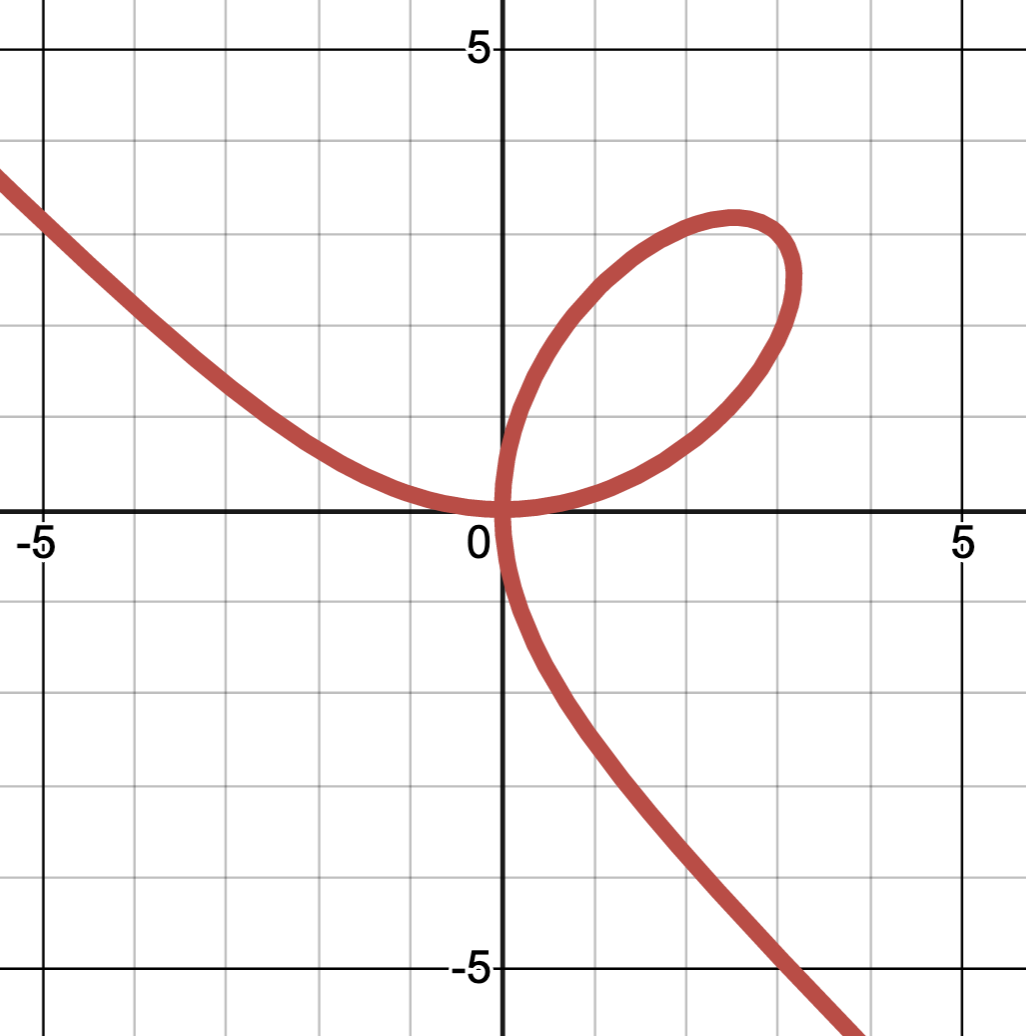
\includegraphics[height=4cm]{fig/descartes}
\index{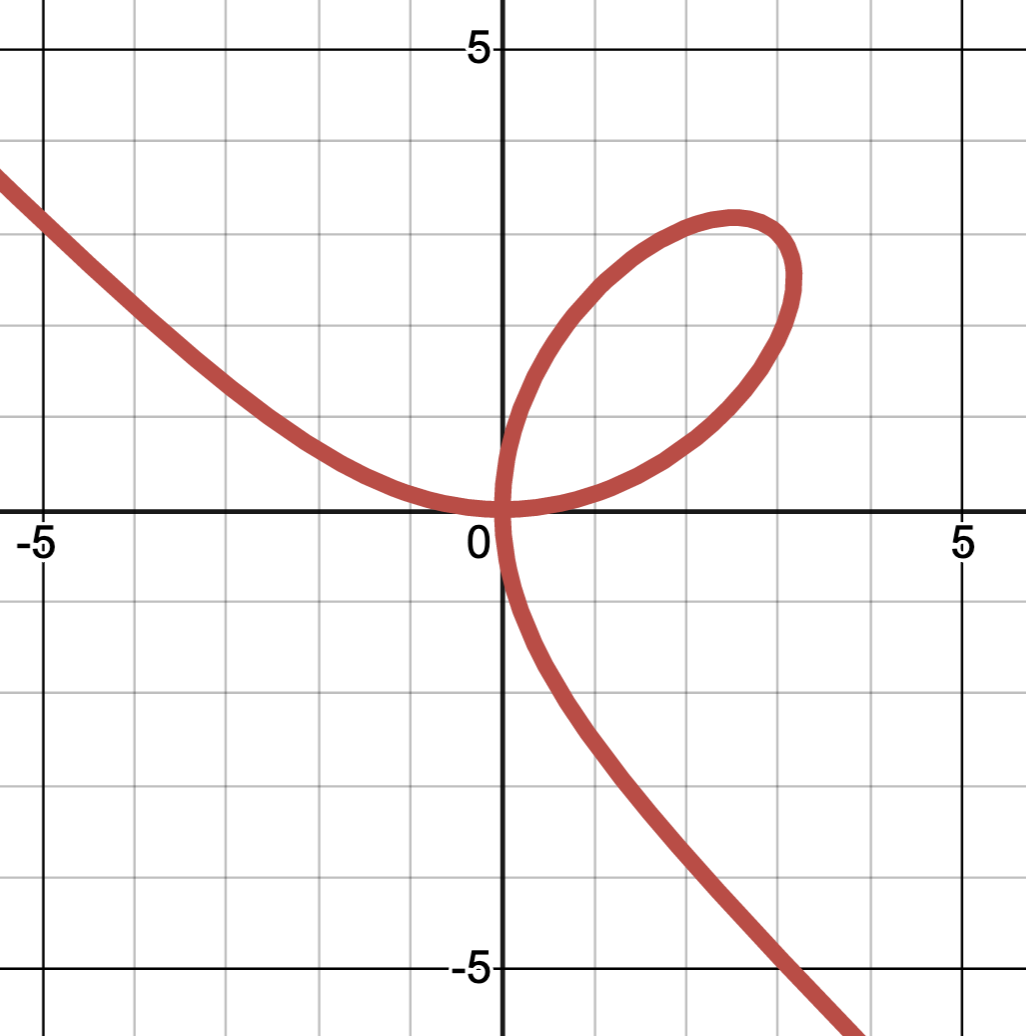
\includegraphics[height=5mm]{fig/descartes} screenshot of graph using Desmos Graphing Calculator, \url{https://www.desmos.com/calculator} (accessed 7 July 2021)}}


\only<2|handout:0>{\color{answercolor}\vfill\small
We know $\frac{dx}{dt}=-2$ when $x=y=3$, and we would like to find $\frac{dy}{dt}$ at the same time. The relationship between $x$ and $y$ is given.
\[x(t)^3+y(t)^3=6x(t)y(t)\] 
We differentiate.
\[3x(t)^2\frac{dx}{dt}(t)+3y(t)^2\frac{dy}{dt}(t)
        =6\left(x(t)\frac{dy}{dt}(t)+y(t)\frac{dx}{dt}(t)\right)\]
When $x(t)=y(t)=3$ and $\diff{x}{t}(t)=-2$,
\[3(9)(-2)+3(9)\frac{dy}{dt}=6\left(3\frac{dy}{dt}+3(-2)\right)\]
\[\frac{dy}{dt}=2\]
So, the roller coaster is moving 2 units per second in the positive $y$ direction.}
\end{frame}
%----------------------------------------------------------------------------------------
%----------------------------------------------------------------
\begin{frame}[t]
\only<1-2>{\QuestionBar{7}{9}\AnswerYes}
\only<1>{\MoreSpace}
\only<3->{\AnswerBar{7}{9}}

\only<1>{Two dogs are tied with elastic leashes to a lamp post that is 2 metres from a straight road. At first, both dogs are on the road, at the closest part of the road to the lamp post. Then, they start running in opposite directions: one dog runs 3 metres per second, and the other runs 2 metres per second. After one second of running, how fast is the angle made by the two leashes increasing?

\begin{center}\begin{tikzpicture}
\draw[thick, double] (-4,0)--(4,0) node[right]{road};
\draw (0,-2) node[vertex, label=below:{lamp post}](p){};
\draw (-3,0) node[vertex, label=above:{doggy 1}](l){};
\draw (2,0) node[vertex, label=above:{doggy 2}](r){};
\draw[thick, C1] (l)--(p)--(r);
\draw[M4] (0.354,-1.65) arc (45:145:.5) node[midway, above]{$\theta$};
\end{tikzpicture}\end{center}}

\only<2-|handout:0>{\footnotesize
Two dogs are tied with elastic leashes to a lamp post that is 2 metres from a straight road. At first, both dogs are on the road, at the closest part of the road to the lamp post. Then, they start running in opposite directions: one dog runs 3 metres per second, and the other runs 2 metres per second. After one second of running, how fast is the angle made by the two leashes increasing?

\begin{tikzpicture}[scale=0.55]
\draw[thick, double] (-4,0)--(4,0) node[right]{road};
\draw (0,-2) node[vertex, label=below:{lamp post}](p){};
\draw (-3,0) node[vertex, label=above:{doggy 1}](l){};
\draw (2,0) node[vertex, label=above:{doggy 2}](r){};
\draw[thick, C1] (l)--(p)--(r);
\onslide<2>{\draw[M4] (0.354,-1.65) arc (45:145:.5) node[midway, above]{$\theta$};}
\onslide<3->{
\draw[thick, dashed, M4] (p)--(0,0);
\draw[black] (-0.4,-1.2) node{$\theta_1$};
\draw[black] (0.32,-1.2) node{$\theta_2$};
}
\end{tikzpicture}}

\only<3-|handout:0>{\color{answercolor}
The angle $\theta$ made by the leashes is made up of $\theta_1+\theta_2$, as shown on either side of the dashed line above. 
\begin{align*}
\tan\big(\theta_1(t)\big) &= \frac{3t}{2}
 \implies\sec^2\big(\theta_1(t)\big) \cdot \theta_1'(t)=\frac{3}{2}
 \implies\theta_1'(t)=\frac{3}{2}\cos^2\big(\theta_1(t)\big) \\
\tan\big(\theta_2(t)\big) &= \frac{2t}{2}
 \implies\sec^2\big(\theta_2(t)\big) \cdot \theta_2'(t)=1
 \implies\theta_2'(t)=\cos^2\big(\theta_2(t)\big)
\end{align*}
At $t=1$,  doggy 1 is three metres away from its starting position and
 doggy 2 is two metres away, so 
$\cos\theta_1=\frac{2}{\sqrt{2^2+3^2}}=\frac{2}{\sqrt{13}}$
and $\cos\theta_2=\frac{2}{\sqrt{2^2+2^2}}=\frac{1}{\sqrt{2}}$ and
\[
\theta_1'=\frac{3}{2}\cos^2\theta_1
         %= \frac{3}{2}\left(\frac{2}{\sqrt{2^2+3^2}}\right)^2
         =\frac{6}{13}\qquad \theta_2'=\cos^2\theta_1
         %=\left(\frac{2}{\sqrt{2^2+2^2}}\right)^2
       =\frac{1}{2}
\] 

So, all together, $\theta'=\theta_1'+\theta_2'
      =\frac{6}{13}+\frac{1}{2}=\frac{25}{26}$ radians per second.
}
\end{frame}
%----------------------------------------------------------------%----------------------------------------------------------------------------------------
\begin{frame}[t]
\unote{Example~\eref{text}{eg_3_2_3}}
\QuestionBar{8}{9}
A \textcolor{C1}{crow} is \textcolor{C1}{one kilometre due east} of the math building, heading \textcolor{C1}{east at 5 kph}. An \textcolor{W2}{eagle} is \textcolor{W2}{two kilometres due north} of the math building, heading \textcolor{W2}{north at 7kph}. How fast is the distance between the two birds increasing at this instant?

\end{frame}
%----------------------------------------------------------------------------------------
%----------------------------------------------------------------------------------------
\begin{frame}<handout:0>[t]
\unote{Example~\eref{text}{eg_3_2_3}}

\color{answercolor}\AnswerBar{8}{9}
\begin{multicols}{2}
\begin{tikzpicture}
\draw[ultra thick] (0,0)--(0,3)node[midway,left]{$y$}--(3,0)node[midway,above]{$D$} -- (0,0) node[midway,below]{$x$};
\draw (0,3) node[above]{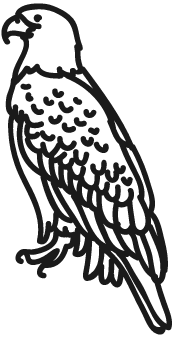
\includegraphics[height=1cm]{Clipart/eagle}};
\draw (3,0) node[right]{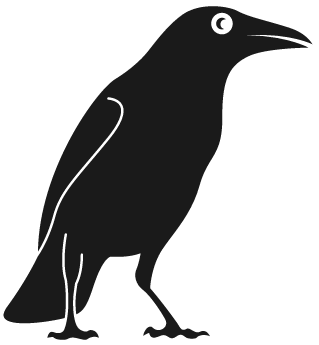
\includegraphics[height=1cm]{Clipart/crow}};
\draw (0,0) node[M4, vertex]{};
\end{tikzpicture}
\index{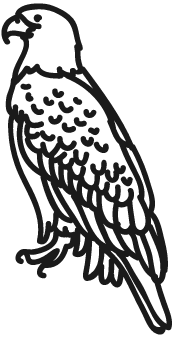
\includegraphics[height=5mm]{Clipart/eagle}
\href{https://thenounproject.com/term/eagle/3575262/}{`Eagle'} by
\href{https://thenounproject.com/heyrabbit/}{Hey Rabbit} is licensed under \CCBYthree~   (accessed 7 July 2021)
}
\index{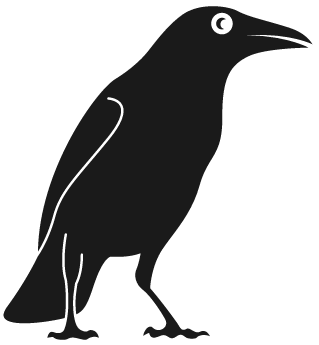
\includegraphics[height=5mm]{Clipart/crow}
\href{https://thenounproject.com/term/crow/1125213/}{`Crow'} by  \href{https://thenounproject.com/sevenknights_friendship/}{Bakunetsu Kaito} is in the
public domain (accessed 7 July 2021) }
\columnbreak

We relate all the variables:
\[D(t)^2=x(t)^2+y(t)^2\]
Differentiate with respect to time:
\[2D(t)\frac{dD}{dt}(t) = 2x(t)\frac{dx}{dt}(t)+2y(t)\frac{dy}{dt}(t)\]

At the time of interest $x=1$, $x'=5$, $y=2$, $y'=7$ and
\[D = \sqrt{x^2+y^2}=\sqrt{1^2+2^2}=\sqrt{5}\]
So
$2\sqrt{5}\frac{dD}{dt}=2(1)(5)+2(2)(7)$.
Then their distance is increasing at $\frac{19}{\sqrt{5}}\approx 8.5$ kph.
\end{multicols}
\end{frame}
%----------------------------------------------------------------------------------------
%----------------------------------------------------------------------------------------
\begin{frame}[t]
\only<1>{\QuestionBar{9}{9}\AnswerYes}
\only<2->{\AnswerBar{9}{9}}
A triangle has one side that is 1cm long, and another side that is 2cm, and the third side is formed by an elastic band that can shrink and stretch. The two fixed sides are rotated so that the angle they form, $\theta$, grows by 1.5 radians each second. Find the rate of change of the area inside the triangle when $\theta=\pi/4$.
\color{answercolor}
\only<2|handout:0>{
\begin{multicols}{2}
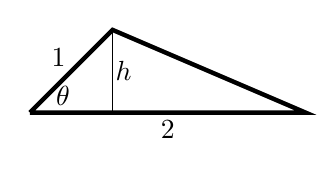
\begin{tikzpicture}[scale=0.7]
\draw[ultra thick] (0,0)--(5,0)--(1.5,1.5)--(0,0);
\draw (2.5,0.2) node[label=below:$2$]{};
\draw (1,1) node[label=left:$1$]{};
\draw (1.5,1.5)--(1.5,0);
\draw (1.7,.75) node{$h$};
\draw (.6,.3) node{$\theta$};
\end{tikzpicture}

$\sin \theta(t) = \frac{opp}{hyp} = \frac{h(t)}{1}=h(t)$, and 

$A(t)=\frac{1}{2}b\,h(t)$,
\columnbreak

So
{\abovedisplayskip=0pt
\begin{align*}
A(t) &= \tfrac{1}{2}(2)\sin \theta(t) = \sin \theta(t)\\
\tfrac{dA}{dt}(t) &= \cos\theta(t) \cdot \tfrac{d\theta}{dt}(t)
\end{align*}
When $\theta=\pi/4$,
\begin{align*}
 \tfrac{dA}{dt} &= \cos(\tfrac\pi4)(1.5) \\
                 &= \tfrac{3}{2\sqrt{2}}
                     \tfrac{\text{cm}^2}{\text{sec}}
\end{align*}}
\end{multicols}}
\end{frame}
%----------------------------------------------------------------------------------------
%----------------------------------------------------------------------------------------

